% !TeX spellcheck = en_US
\section{Application overview}\label{section:overview}

In this chapter we will provide general overview of main application window.

\begin{figure*}[!ht] 
	\centering
	\makebox[\textwidth]{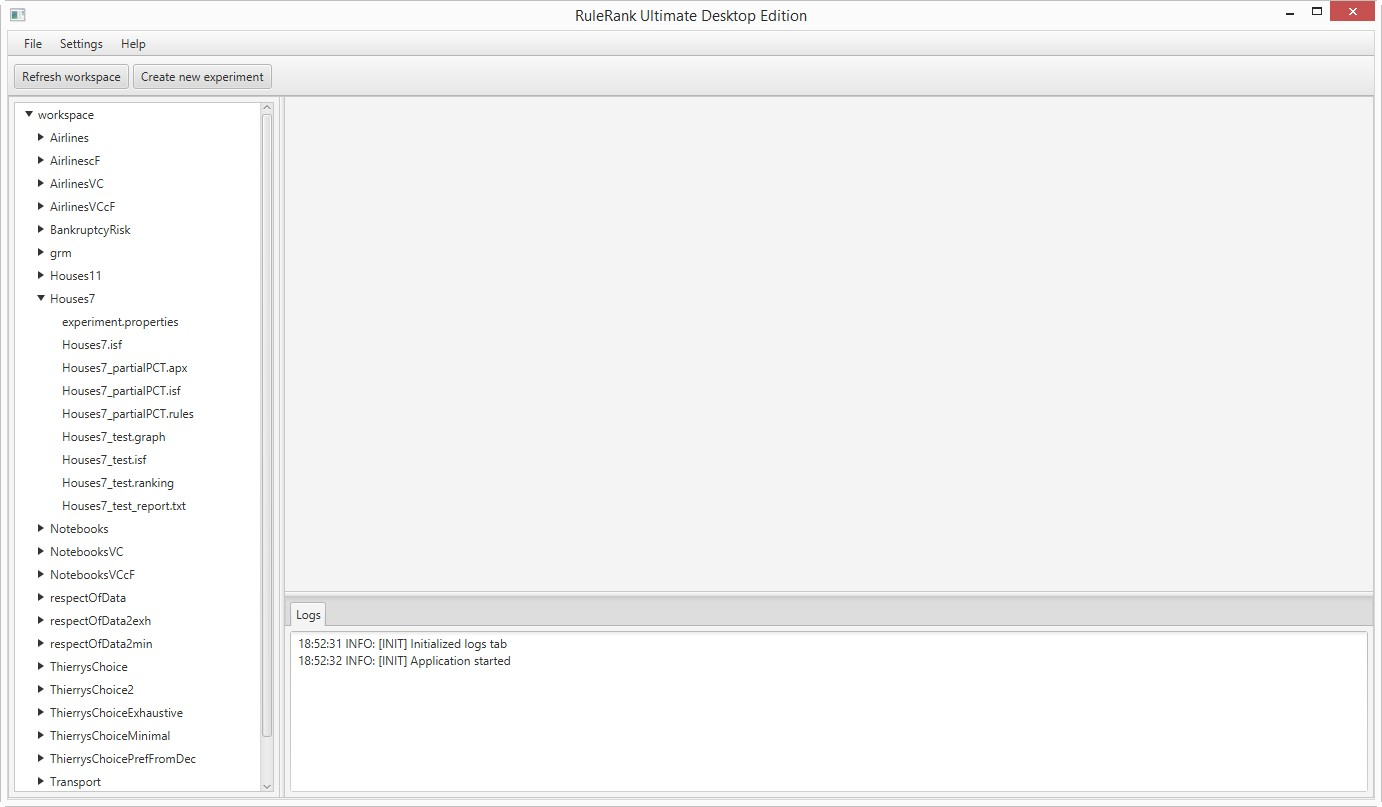
\includegraphics[width=.7\paperwidth]{overview}}
	\caption{Main window screen}
\end{figure*}

There are three main panels in RUDE application:
\begin{itemize}
	\item workspace(1) - it manages all files
	\item upper panel(2) - it displays most of the information. It can display multiple tabs like web browser. Most of the work will be done here.
	\item lower panel(3) - it contains logs and can display additional information for some upper tabs. It can display multiple tabs like web browser.
\end{itemize}

On top of main window you can find menu:
\begin{itemize}
	\item File - it currently enables to quit program
	\item Settings - it contains user settings for RUDE application
	\item Help - it contains About and Help modal dialogs.
\end{itemize}

Below menu you can find toolbar with actions, with will be described in \hyperref[section:workspace]{Workspace management section}.\\


\textbf{Logs tab:}\\
Logs tab display all logs from application. 
Currently there are three logs levels:
\begin{itemize}
	\item INFO - displays some useful information about performed actions
	\item WARN - indicates some misconfiguration or action aborting in certain conditions. It also indicates errors handled by application.
	\item ERROR - displays errors not handled properly by application
\end{itemize}

Logs can be copied by selecting text and pressing Ctrl + C. All logs can be clear by right clicking on logs panel and choosing "Clear logs" option.

\vfill\newpage